
%% bare_jrnl_compsoc.tex
%% V1.4a
%% 2014/09/17
%% by Michael Shell
%% See:
%% http://www.michaelshell.org/
%% for current contact information.
%%
%% This is a skeleton file demonstrating the use of IEEEtran.cls
%% (requires IEEEtran.cls version 1.8a or later) with an IEEE
%% Computer Society journal paper.
%%
%% Support sites:
%% http://www.michaelshell.org/tex/ieeetran/
%% http://www.ctan.org/tex-archive/macros/latex/contrib/IEEEtran/
%% and
%% http://www.ieee.org/

%%*************************************************************************
%% Legal Notice:
%% This code is offered as-is without any warranty either expressed or
%% implied; without even the implied warranty of MERCHANTABILITY or
%% FITNESS FOR A PARTICULAR PURPOSE! 
%% User assumes all risk.
%% In no event shall IEEE or any contributor to this code be liable for
%% any damages or losses, including, but not limited to, incidental,
%% consequential, or any other damages, resulting from the use or misuse
%% of any information contained here.
%%
%% All comments are the opinions of their respective authors and are not
%% necessarily endorsed by the IEEE.
%%
%% This work is distributed under the LaTeX Project Public License (LPPL)
%% ( http://www.latex-project.org/ ) version 1.3, and may be freely used,
%% distributed and modified. A copy of the LPPL, version 1.3, is included
%% in the base LaTeX documentation of all distributions of LaTeX released
%% 2003/12/01 or later.
%% Retain all contribution notices and credits.
%% ** Modified files should be clearly indicated as such, including  **
%% ** renaming them and changing author support contact information. **
%%
%% File list of work: IEEEtran.cls, IEEEtran_HOWTO.pdf, bare_adv.tex,
%%                    bare_conf.tex, bare_jrnl.tex, bare_conf_compsoc.tex,
%%                    bare_jrnl_compsoc.tex, bare_jrnl_transmag.tex
%%*************************************************************************


% *** Authors should verify (and, if needed, correct) their LaTeX system  ***
% *** with the testflow diagnostic prior to trusting their LaTeX platform ***
% *** with production work. IEEE's font choices and paper sizes can       ***
% *** trigger bugs that do not appear when using other class files.       ***                          ***
% The testflow support page is at:
% http://www.michaelshell.org/tex/testflow/


\documentclass[10pt,conference,onecolumn,compsoc]{IEEEtran}


\usepackage{hyperref}
\usepackage{enumitem}
\setlist[itemize]{leftmargin=3 cm}
\setlist[enumerate]{leftmargin=3cm}



% *** CITATION PACKAGES ***
%
\ifCLASSOPTIONcompsoc
  % IEEE Computer Society needs nocompress option
  % requires cite.sty v4.0 or later (November 2003)
  \usepackage[nocompress]{cite}
\else
  % normal IEEE
  \usepackage{cite}
\fi
% cite.sty was written by Donald Arseneau
% V1.6 and later of IEEEtran pre-defines the format of the cite.sty package
% \cite{} output to follow that of IEEE. Loading the cite package will
% result in citation numbers being automatically sorted and properly
% "compressed/ranged". e.g., [1], [9], [2], [7], [5], [6] without using
% cite.sty will become [1], [2], [5]--[7], [9] using cite.sty. cite.sty's
% \cite will automatically add leading space, if needed. Use cite.sty's
% noadjust option (cite.sty V3.8 and later) if you want to turn this off
% such as if a citation ever needs to be enclosed in parenthesis.
% cite.sty is already installed on most LaTeX systems. Be sure and use
% version 5.0 (2009-03-20) and later if using hyperref.sty.
% The latest version can be obtained at:
% http://www.ctan.org/tex-archive/macros/latex/contrib/cite/
% The documentation is contained in the cite.sty file itself.



% *** GRAPHICS RELATED PACKAGES ***
%
\ifCLASSINFOpdf
   \usepackage[pdftex]{graphicx}
 
\else
 
\fi
% graphicx was written by David Carlisle and Sebastian Rahtz. It is
% required if you want graphics, photos, etc. graphicx.sty is already
% installed on most LaTeX systems. The latest version and documentation
% can be obtained at: 
% http://www.ctan.org/tex-archive/macros/latex/required/graphics/
% Another good source of documentation is "Using Imported Graphics in
% LaTeX2e" by Keith Reckdahl which can be found at:
% http://www.ctan.org/tex-archive/info/epslatex/
%
% latex, and pdflatex in dvi mode, support graphics in encapsulated
% postscript (.eps) format. pdflatex in pdf mode supports graphics
% in .pdf, .jpeg, .png and .mps (metapost) formats. Users should ensure
% that all non-photo figures use a vector format (.eps, .pdf, .mps) and
% not a bitmapped formats (.jpeg, .png). IEEE frowns on bitmapped formats
% which can result in "jaggedy"/blurry rendering of lines and letters as
% well as large increases in file sizes.
%
% You can find documentation about the pdfTeX application at:
% http://www.tug.org/applications/pdftex









% *** PDF, URL AND HYPERLINK PACKAGES ***
%
\usepackage{url}
% url.sty was written by Donald Arseneau. It provides better support for
% handling and breaking URLs. url.sty is already installed on most LaTeX
% systems. The latest version and documentation can be obtained at:
% http://www.ctan.org/tex-archive/macros/latex/contrib/url/
% Basically, \url{my_url_here}.




\begin{document}

\title{Deliverable for UltraWeather\\ for UTM CSCI 352}
%
%

% received ..."  text while in non-compsoc journals this is reversed. Sigh.

\author{Andrew Newbill, Joshua Chamberlain, Aaron Alden\\ % <-this % stops a space
}

\IEEEtitleabstractindextext{%
\begin{abstract}
This computer application uses a weather API to collect certain weather data such as temperature, humidity, etc. to predict the weather forecast throughout 
the day. The target audience are driving adults who need to know the weather conditions to get to work on time. The application will also have emergency notifications, such as tornado warnings. The progress on the project is that we have selected a specific API to collect weather data.
\end{abstract}

}


% make the title area
\maketitle



\IEEEdisplaynontitleabstractindextext

\IEEEpeerreviewmaketitle



\section{Introduction}
\quad We planned this project as a way to practice our C\# and design pattern skills. Our hope is that in doing so we can deliver a product that is user friendly and well designed so that users will have an easy way to check the weather from their desktop. One advantage of this is that web browsers are often resource hungry and a small WPF app like ours will not be. This is crucial for low end systems where multitasking with a web-browser open slows everything to a crawl. We are really targeting power-users who would like to use as little resources as possible to track the weather for as many areas as they choose. It is often the case with weather apps that they quickly become cumbersome when used for more than a few cities/regions.

\quad Another issue we plan to tackle with this project is privacy. Weather applications by companies such as Apple almost certainly store your information on a server. Since most people keep not only the city they live in but the ones that they travel to pinned in these apps, Apple knows exactly where you live and where you go based off only in the information in this application. By storing this information client-side(and we plan to encrypt it) we give the user more security in how their data is stored. Closed ecosystems such as Apple's intentionally do not reveal exactly how they handle user information and this is not acceptable to everyone. We intend to be entirely transparent about how we handle your data since the project will be open-sourced once it is delivered. Even if our implementation ends up being imperfect or less secure than we hoped, at least we won't be hiding it.


%Your introduction should give an introduction to your project.  What are you trying to %accomplish (high level), who do you expect to target with your project?  What do you expect %your target audience will get out of it?

%Should you need to cite anything, use the \emph{cite} keyword, and refer to something from your %bibliography.  For example, this was put together with the help of a \LaTeX guide%\cite{IEEEhowto:kopka}.


%Make sure that by the end of your introduction the reader knows what your project is and why you are doing it.



%\subsection{Subsection Heading Here}
%Occasionally you need to break your sections into separate parts, you will likely not need a %subsection for every section

% needed in second column of first page if using \IEEEpubid
%\IEEEpubidadjcol

%\subsubsection{Subsubsection Heading Here}
%Occasionally you will need to break your subsections into separate parts, if you find yourself %using this often, you're likely going overboard.  Don't try to go any lower down than this. %(And make sure you remove this!)



\subsection{Background}
\subsubsection{Terms to Know}
	The reader should be familiar with the general terms used to refer to various weather patterns. We plan to use a tiling system for this project. A tile in the context of our program will be a drag-able object that contains information on the weather for specific city or town.
You will be able to organize these tiles with folders, which are simply containers for tiles. 
\subsubsection{Personal Connection}	
	 We came up with the idea for this project because most weather apps are integrated into operating systems and as such they have limited functionality for users who may travel between large areas or are simply interested in following the weather on a large scale. One strong inspiration was the recently unpredictable weather in Tennessee. It would be good for users working on the desktop to be able to check the weather as they work with a simple and fast app that does not run as a system service. 
%In this section, give a brief background to any concepts the reader may need to know to make it %through your paper.   Are there any specific terms the reader needs to be familiar with?

%Also, consider going into your personal connection with this project -- why did you decide to do %it?

\subsection{Impacts}
%In this section, you should be attempting to judge the broader impact of your work, %specifically impacts on: public health, safety, and welfare, as well as global, cultural, %social, environmental, and economic factors.  While your project likely does not have any %impact on all of the above, try to consider and evaluate how your project will impact society %and the world at large (even if only in a very small way).
We hope that our project we impact the safety of its users in a positive way. A user could be working at their computer, blissfully unaware of a coming storm. We hope that our user would happen to check the app and decide not to leave their home on that day. This common situation could also impact the safety of the general public since more people on the road during a dangerous storm leads to a higher chance of accidents. It could happen that a social get-together that was planned gets canceled once one user sees coming poor weather and notifies their friends. We also hope that working on this project impacts us positively by furthering our experience at proposing projects and working as a group.  	



\subsection{Challenges}
	The first major challenge will be getting a C\# WPF application to interact with the OpenWeather API. Once we can call the api and receive data the next major challenge will be organizing this data into something that is easy for the user to view and interpret. After that we will have to overcome the task of implementing 'tiles' that allow the user to organize more than one location's data. We plan to overcome the challenges by first reading the XML data into variables that can be married to fields in the tiles. Getting the data organized into something that is pleasant to view and organize will be by far the biggest challenge of this project. The free tier of OpenWeather does have certain limitations


\section{Scope}
	We understand that in 2022, most weather apps have the same features we come to expect. The main way we can make our app different is by focusing more on the aesthetics and graphics of the app. We want to take a minimalist, tile approach to our app. We also want to implement our radar. Whether we will have it dynamic (a looping map) or static is still to be decided. For our stretch goals, we want to implement severe weather alerts and also "pre-alerts". For the pre-alerts, the idea is to give users a heads-up alert up to a week before severe weather occurs. For example, if meteorologists are predicting a nasty storm front next week, the user should be alerted that there is the possibility for severe weather. Sometimes, just a tornado warning pushed to your phone as the storm is happening is too late to seek shelter.


\subsection{Requirements}
The requirements were acquired with all of us talking in class about the function and non-functional requirements as well as further communication through discord about both types of requirements.

\subsubsection{Functional}
\begin{itemize}
\item The User should have the ability to pick what location they want to get the weather from -- allows the User to get particular information for their use.
\item The User will be able to see all weather information provided by OpenWeatherAPI.
\item The User will be alerted when the national weather service has alerts for the searched location.
\item The system will connect to the OpenWeatherAPI.
\item The User will be able to put locations into folders.
\item The User will be able to search for a location.
\end{itemize}

\subsubsection{Non-Functional}
\begin{itemize}
\item Privacy - The user's search locations will be protected and not given to any third parties.
\item Reliability - The app will work with a proper internet connection.
\item Capacity - The app will have the same capacity as the storage on the computer i.e. The user will be able to have as many locations as their phone or computer can fit. Also the API calls are limited to 1,000,000 calls per month.
\end{itemize}

\subsection{Use Cases}


\begin{table}
\centering
\begin{tabular}{|c|c|c|c|c|}
\hline
Use Case ID & Use Case Name & Primary Actor & Complexity & Priority \\
\hline \hline
1 & Set location & Application user & Med & 1\\
\hline
2 & Add Favorites & Application user & Low & 2\\
\hline
3 & Search Location's weather & Application user & Med & 3\\
\hline

\end{tabular}
\caption{UltraWeather 1st draft use case table}
\label{tab:useCaseIndex}
\end{table}

\begin{itemize}
\item[Use Case Number:] 1
\item[Use Case Name:] Set location
\item[Description:] Upon opening the application, the user will have the option to set their current location, i.e. ``Use current location". The user will then be presented with the weather forecast for the provided location.
\end{itemize}

\begin{enumerate}
\item If the user wishes the application to find their location, they will click on the alert that the application is trying to access their location.
\item If the user wishes to set their home location manually, they can enter their zip code into a ``Set your location" menu option.
\item[Termination Outcome:] The user now has access to their ``home" location's weather. Making it readily available whenever they access the application.
\end{enumerate}

\begin{itemize}
\item[Use Case Number:] 2
\item[Use Case Name:] Add favorites
\item[Description:] The user can store favorite places to readily see what the weather is for these saved locations. They will be collected all in one place.
\end{itemize}

\begin{enumerate}
\item The user will navigate to ``Add favorites" section.
\item The user will type in the zip code for desired location.
\item The user will have the option to save as a favorite to be readily available to view.
\item[Termination Outcome:] A collection of saved favorite locations will be stored in the application.
\end{enumerate}

\begin{itemize}
\item[Use Case Number:] 3
\item[Use Case Name:] Search Location's weather
\item[Description:] The user will have the option to search for a location's weather by location (zip code). The application will then show them the current weather forecast for the searched location. 
\end{itemize}

\begin{enumerate}
\item The user will type in the desired City into the textbox and select a state from the combobox. Then they will press a button and the data will appear for that city.
\item The application will present the current weather forecast.
\item The user can search for new locations if desired. 
\item[Termination Outcome:] The user can now interact with all features of the application regarding this location.
\end{enumerate}

\subsection{Interface Mockups}
\begin{figure}[ht!]
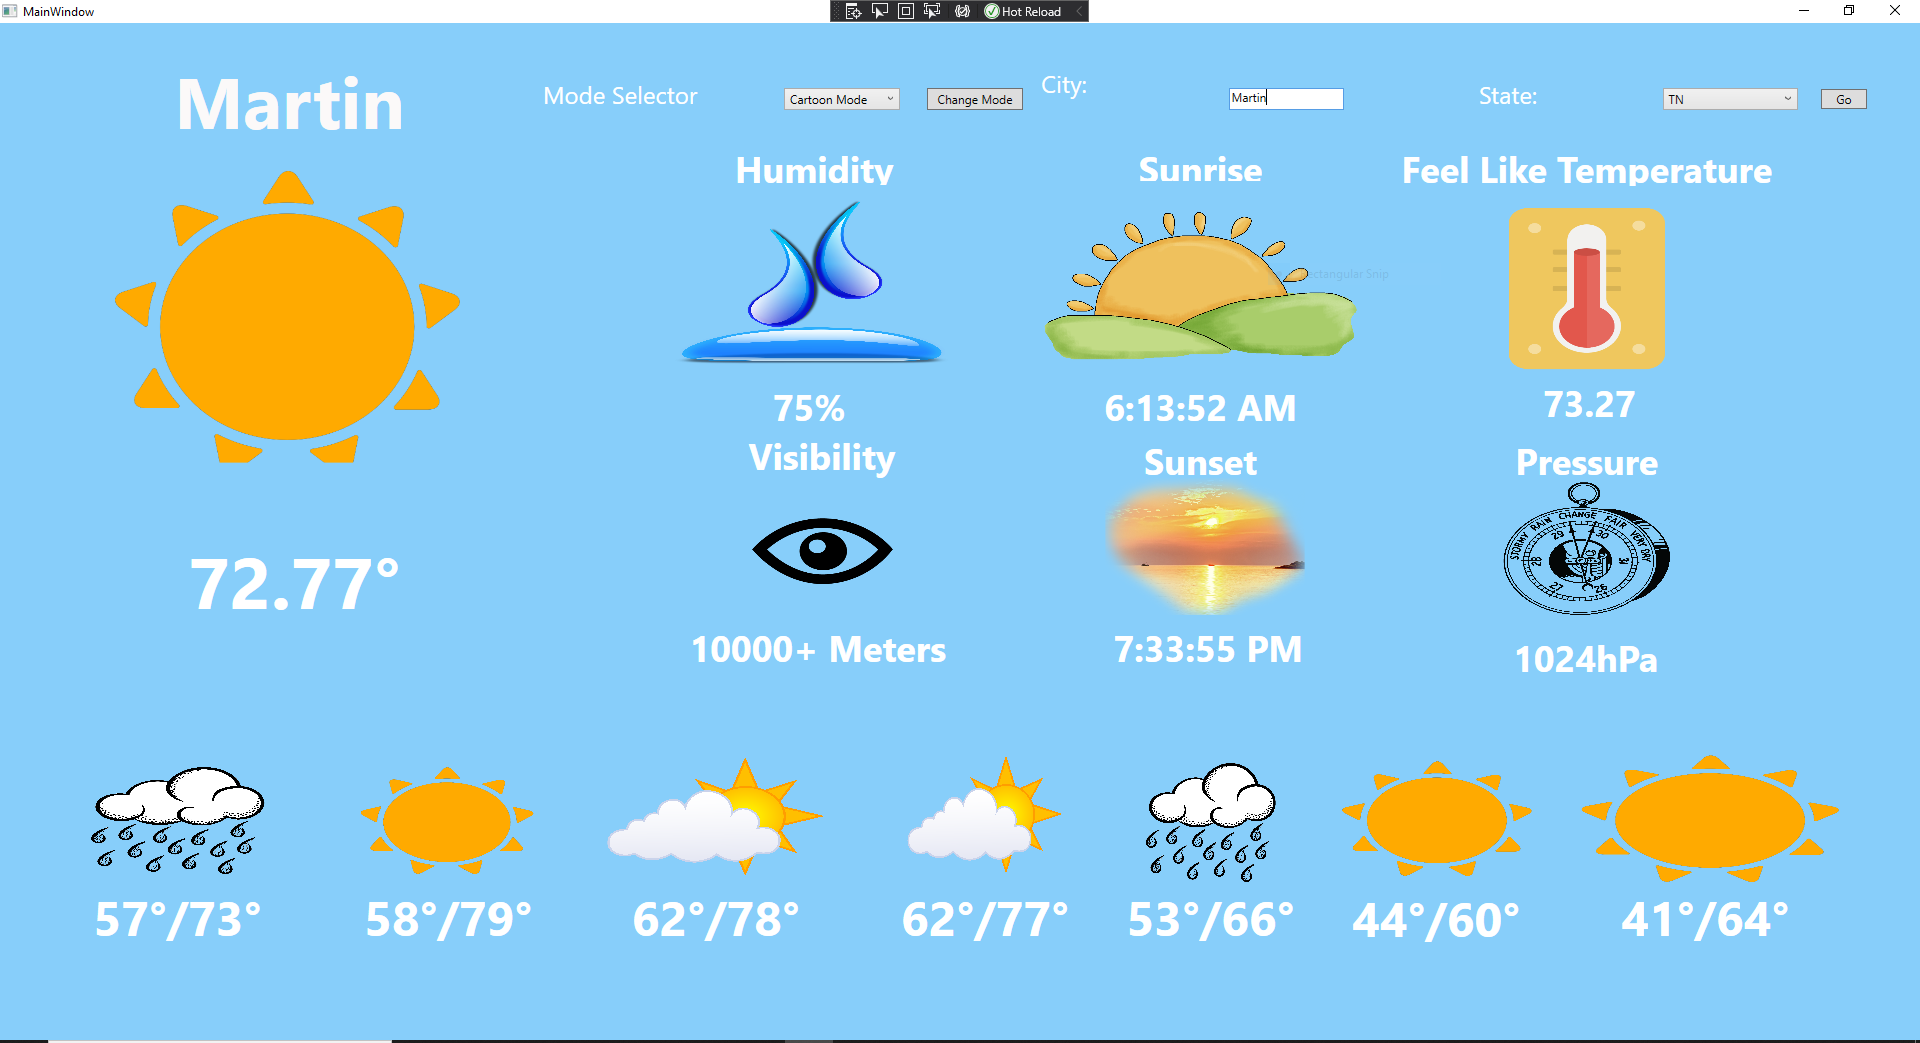
\includegraphics[scale=0.3]{use_case_1.png}
\caption{Illustration of Use Case 1. Here the user is choosing whether or not to automatically obtain their location.}
\label{use_case_1}
\end{figure}

\begin{figure}[ht!]
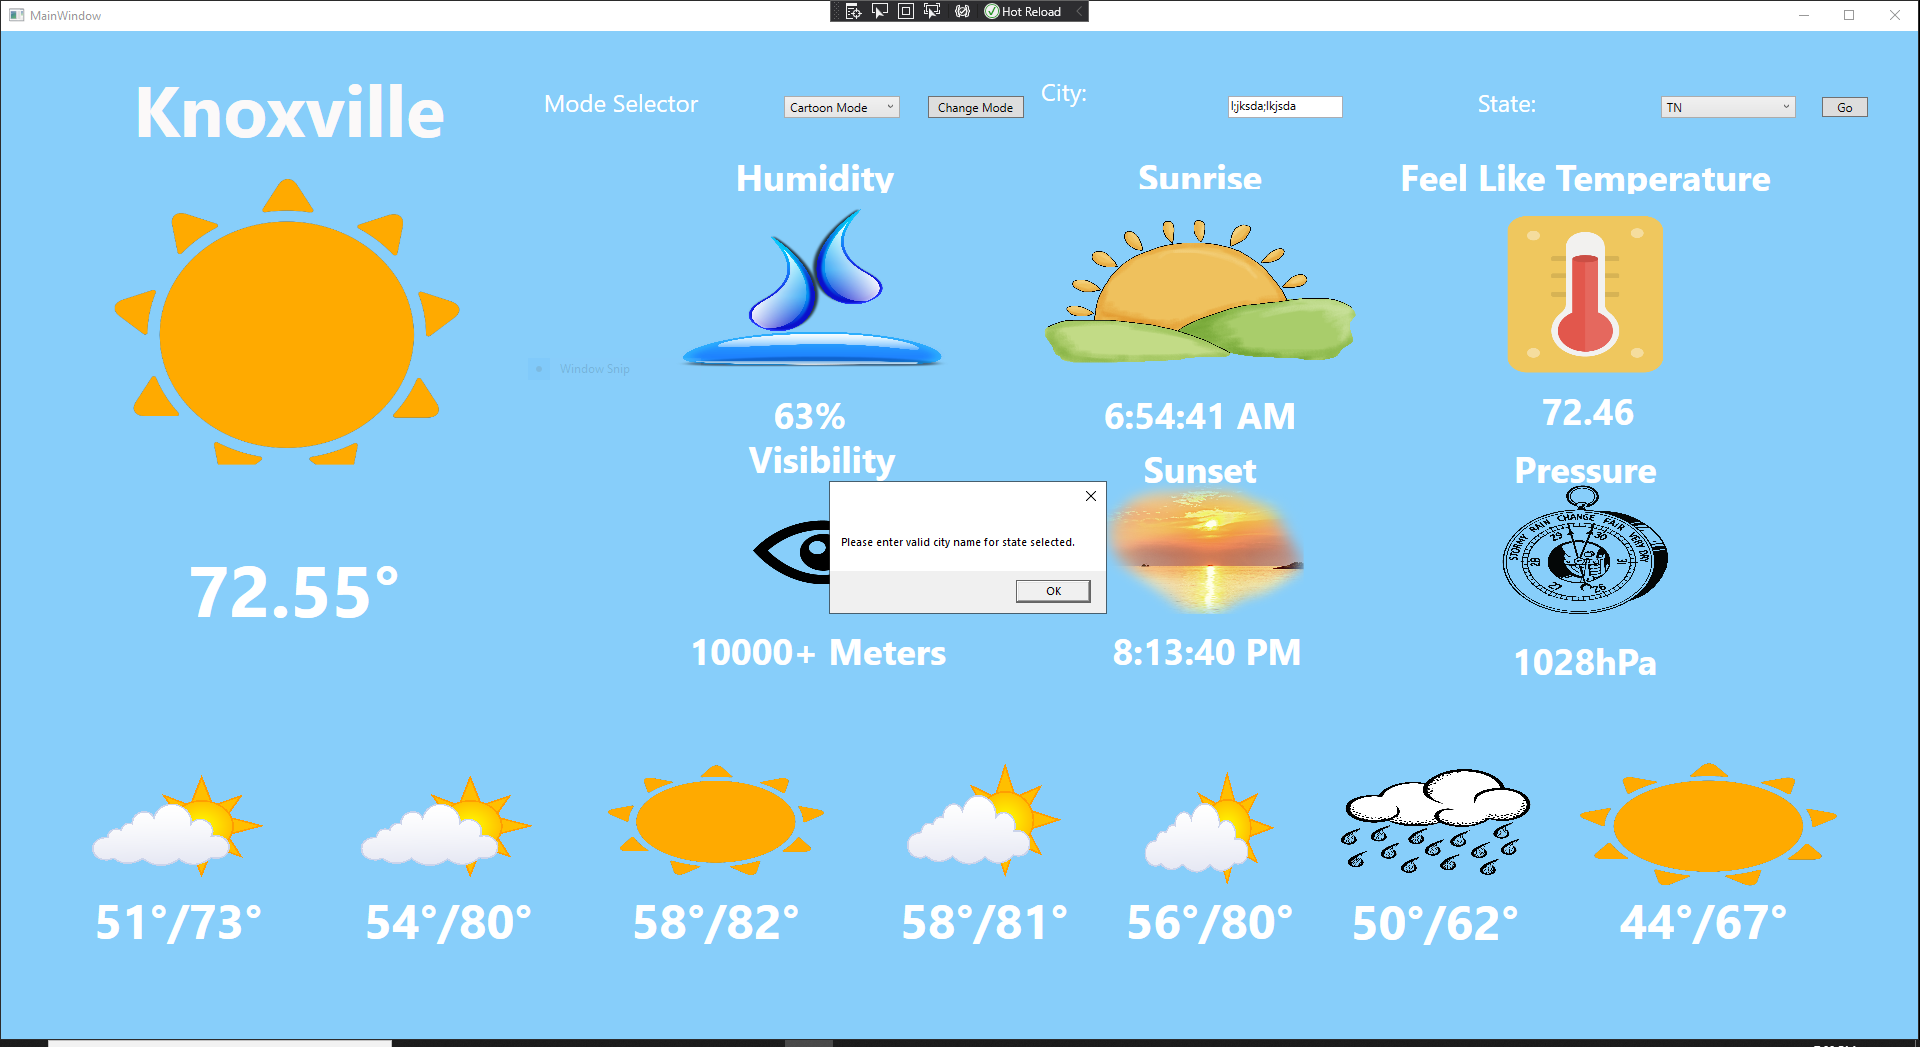
\includegraphics[scale=0.3]{use_case_2.png}
\caption{Illustration of Use Case 2. Here the user is adding a favorite to their favorites folder.}
\label{use_case_2}
\end{figure}

\begin{figure}[ht!]
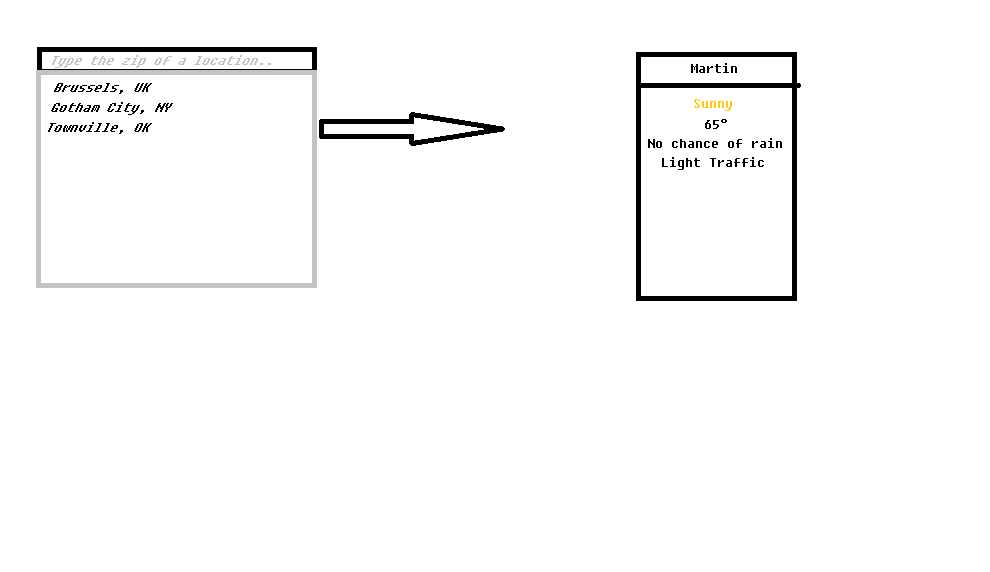
\includegraphics[scale=0.3]{use_case_3.png}
\caption{Illustration of Use Case 3. Here the user is searching for a location.}
\label{use_case_3}
\end{figure}


\section{Project Timeline}
\begin{figure}[ht !]
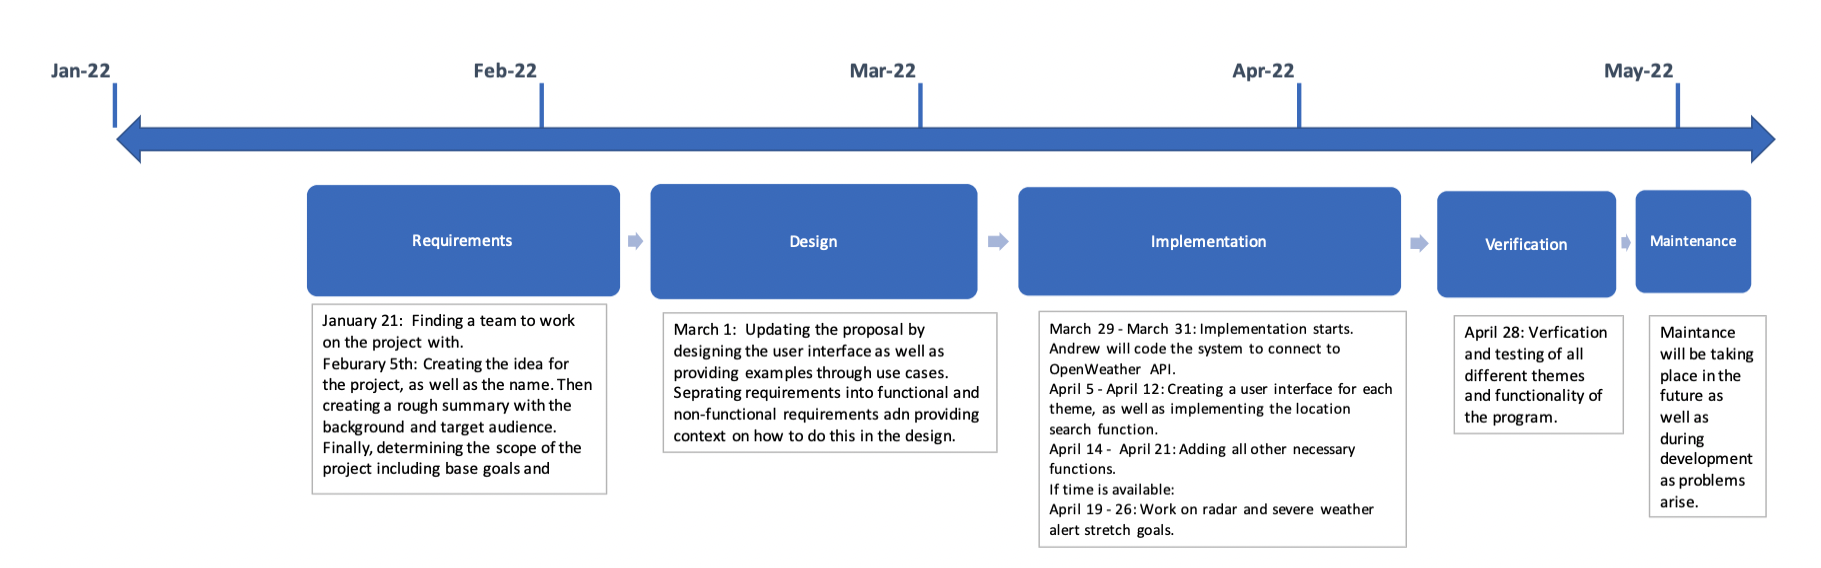
\includegraphics[scale = 0.5]{Timeline.png}
\caption{Full Project Timeline}
\label{TimeLine}
\end{figure}
Milestones:
Feburary 5th: The requirements stage has been discussed and decided.
March 1st: All designs are finished, shown through our use cases.
March 29 - 31: Implementation starts with Andrew coding the system that connects to the API.
April 5 - 12: Implementing the user interface designs shown through the use cases and implementing the location search function.
April 14 - 21: Implementing other functions such as the tiling system and GPS optimal route searching functions
If time is available:
April 19 - 26: Work on radar stretch goal.
April 28: Verfication and testing of all different themes and functionality of the program.
Maintance will be taking place in the future as well as during development as problems arise.

\subsection{UML Outline}
\begin{figure}[ht!]
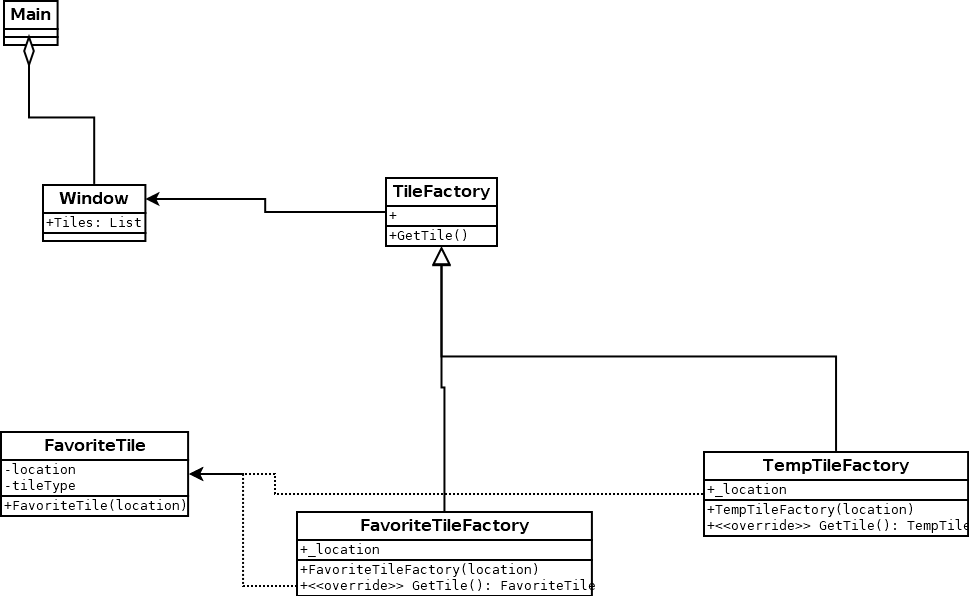
\includegraphics[scale = 0.3]{WeatherApp.png}
\end{figure}

\section{Project Structure}
We haven't decided on all of design patterns yet but we feel that the factory method would be good for the tile system we plan to implement. Each factory will be responsible for producing different types of tile, depending on what the users wants. We also need to come up with some more tile types to make the project more useful and compelling to use.




\subsection{Design Patterns Used}
We used a facade pattern and a vistor pattern. The facade pattern comes with the user interface. The user interface is set up in a way that the user can provide information to the system, but they cannot touch anything on the backend. The visitor pattern is used when checking the mode/theme of the program. The program visits each data point (the two themes in this case) and does different actions based on which one it is. 


\section{Results}
The UltraWeather collects data from OpenWeather API and displays it to the screen in a user friendly way. UltraWeather allows the person to type in a city and checks whether the city is valid. It provides an error MessageBox when it is not valid. The pictures will change when the weather is different, and the forecast will be as accurate as the API.

\subsection{Future Work}
Where are you going next with your project?
For early deliverables, what are your next steps?  (HINT: you will typically want to look back at your timeline and evaluate: did you meet your expected goals?  Are you ahead of schedule?  Did you decide to shift gears and implement a new feature?)
By the end, what do you plan on doing with this project?  Will you try to sell it?  Set it on fire?  Link to it on your resume and forget it exists?




\begin{thebibliography}{1}

\bibitem{IEEEhowto:kopka}
H.~Kopka and P.~W. Daly, \emph{A Guide to \LaTeX}, 3rd~ed.\hskip 1em plus
  0.5em minus 0.4em\relax Harlow, England: Addison-Wesley, 1999.

\end{thebibliography}



\begin{IEEEbiography}{Michael Shell}
Biography text here.
\end{IEEEbiography}

% if you will not have a photo at all:
\begin{IEEEbiographynophoto}{John Doe}
Biography text here.
\end{IEEEbiographynophoto}

% insert where needed to balance the two columns on the last page with
% biographies
%\newpage

\begin{IEEEbiographynophoto}{Jane Doe}
Biography text here.
\end{IEEEbiographynophoto}





% that's all folks
\end{document}


